\documentclass[twoside]{article}
\setlength{\oddsidemargin}{0.25 in}
\setlength{\evensidemargin}{-0.25 in}
\setlength{\topmargin}{-0.6 in}
\setlength{\textwidth}{6.5 in}
\setlength{\textheight}{8.5 in}
\setlength{\headsep}{0.75 in}
\setlength{\parindent}{0 in}
\setlength{\parskip}{0.1 in}

\usepackage{graphicx}
\usepackage{url}
\usepackage{float}

%
% The following commands sets up the lecnum (lecture number)
% counter and make various numbering schemes work relative
% to the lecture number.
%
\newcounter{lecnum}
\renewcommand{\thepage}{\thelecnum-\arabic{page}}
\renewcommand{\thesection}{\thelecnum.\arabic{section}}
\renewcommand{\theequation}{\thelecnum.\arabic{equation}}
\renewcommand{\thefigure}{\thelecnum.\arabic{figure}}
\renewcommand{\thetable}{\thelecnum.\arabic{table}}
\newcommand{\dnl}{\mbox{}\par}

%
% The following macro is used to generate the header.
%
\newcommand{\lecture}[4]{
  \pagestyle{myheadings}
  \thispagestyle{plain}
  \newpage
  \setcounter{lecnum}{#1}
  \setcounter{page}{1}
  \noindent
  \begin{center}
  \framebox{
     \vbox{\vspace{2mm}
   \hbox to 6.28in { {\bf COMPSCI~590S~~~Systems for Data Science
                       \hfill Fall 2016} }
      \vspace{4mm}
      \hbox to 6.28in { {\Large \hfill Lecture #1: #2  \hfill} }
      \vspace{2mm}
      \hbox to 6.28in { {\it Lecturer: #3 \hfill Scribe(s): #4} }
     \vspace{2mm}}
  }
  \end{center}
  \markboth{Lecture {#1}: #2}{Lecture {#1}: #2}
  \vspace*{4mm}
}

%
% Convention for citations is authors' initials followed by the year.
% For example, to cite a paper by Leighton and Maggs you would type
% \cite{LM89}, and to cite a paper by Strassen you would type \cite{S69}.
% (To avoid bibliography problems, for now we redefine the \cite command.)
%
\renewcommand{\cite}[1]{[#1]}

% \input{epsf}

%Use this command for a figure; it puts a figure in wherever you want it.
%usage: \fig{NUMBER}{FIGURE-SIZE}{CAPTION}{FILENAME}
\newcommand{\fig}[4]{
           \vspace{0.2 in}
           \setlength{\epsfxsize}{#2}
           \centerline{\epsfbox{#4}}
           \begin{center}
           Figure \thelecnum.#1:~#3
           \end{center}
   }

% Use these for theorems, lemmas, proofs, etc.
\newtheorem{theorem}{Theorem}[lecnum]
\newtheorem{lemma}[theorem]{Lemma}
\newtheorem{proposition}[theorem]{Proposition}
\newtheorem{claim}[theorem]{Claim}
\newtheorem{corollary}[theorem]{Corollary}
\newtheorem{definition}[theorem]{Definition}
\newenvironment{proof}{{\bf Proof:}}{\hfill\rule{2mm}{2mm}}

% Some useful equation alignment commands, borrowed from TeX
\makeatletter
\def\eqalign#1{\,\vcenter{\openup\jot\m@th
 \ialign{\strut\hfil$\displaystyle{##}$&$\displaystyle{{}##}$\hfil
     \crcr#1\crcr}}\,}
\def\eqalignno#1{\displ@y \tabskip\@centering
 \halign to\displaywidth{\hfil$\displaystyle{##}$\tabskip\z@skip
   &$\displaystyle{{}##}$\hfil\tabskip\@centering
   &\llap{$##$}\tabskip\z@skip\crcr
   #1\crcr}}
\def\leqalignno#1{\displ@y \tabskip\@centering
 \halign to\displaywidth{\hfil$\displaystyle{##}$\tabskip\z@skip
   &$\displaystyle{{}##}$\hfil\tabskip\@centering
   &\kern-\displaywidth\rlap{$##$}\tabskip\displaywidth\crcr
   #1\crcr}}
\makeatother

% **** IF YOU WANT TO DEFINE ADDITIONAL MACROS FOR YOURSELF, PUT THEM HERE:



% Some general latex examples and examples making use of the
% macros follow.

\begin{document}

%FILL IN THE RIGHT INFO.
%\lecture{**LECTURE-NUMBER**}{**DATE**}{**LECTURER**}{**SCRIBE**}
\lecture{1}{Frequency and Memory Scaling in CPUs}{Emery Berger}{Amber Madvariya, Anish Pimpley}

\section{Introduction}

Modern machines can have multiple CPUs, with each CPU having multiple cores. When Multi-core processors were invented, we saw a squared increase (1-2-4) in the number of cores over a fixed interval of time.\\
Computer Scientists at the time hypothesized that this exponential increase in cores could be extrapolated to the future, and that that we would see hundreds and thousands of cores in machines eventually. We now know that machine certainly did not follow such a trend.\\
\section{Moore's law and Denard scaling:}
\begin{figure}[H]
\centering
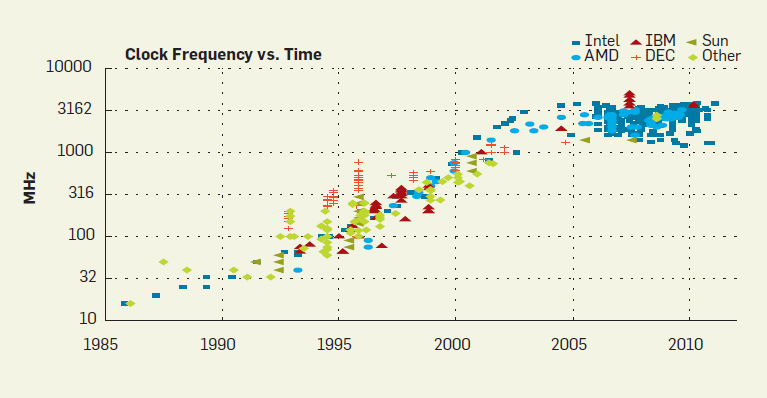
\includegraphics[scale=0.35]{freq.jpg}
\caption{CPU frequency scaling over the years}
\end{figure}\\
As can be seen for the above image, we saw an exponential increase in CPU frequencies with time. This directly related to what was colloquially referred to as Moore's law through a relationship referred to as Denard scaling.\\
\textbf{Moore's law:} The number of transistors in a CPU doubled every 18 months.\\
As the size of the chip remained the same and transistors doubled, the distance between them decreased. This caused propagation delays to decrease and clock speeds to proportionally increase. This observation was formalized in the form of Denard scaling.\\
\textbf{Denard scaling:} Clock speed is linearly related to the number of transistors.\\
\\
Thus, we believed that clock speed would keep doubling every couple of years. This trend was the norm through the 80s and the 90s. It was common for industries to simply wait for computational power to double instead of investing in improving efficiency on the older machine.\\
\\
\section{Synchronous vs Asynchronous systems:}\\
The clock for modern chips operates synchronously in a peak-flat format. Asynchronous systems never caught on. The primary reason for their lack of popularity as the difficulty in fixing bugs. Hardware manufacturers are very sensitive to bugs in CPU hardware. Intel having a bug in its implementation of the division function was one such notorious episode.\\
Post 2000, CPU frequencies stopped scaling and have completely come to a halt for the last decade. Contrary to what it might seem, Moore's law is still very much alive despite this trailing off of CPU frequencies. Moore's law will continue scaling until we reach a point where transistors can't physically maintain 2 charges separately. While we will eventually reach such a point, it is still far in the future. \\
\section{End of exponential scaling in CPU frequency:}\\
The relationship between frequency and transistor size was conditioned on Denard scaling being true. However, a linear increase in frequency corresponded to a squared increase in power consumption with in turn was directly proportional to the heat output. This squared increase in heat emission quickly became unsustainable and we hit a wall for CPU clock speeds, beyond which heat dissipation in standard environments was not feasible. Denard scaling can thus be considered dead in the present day. For reference, if Denard scaling held true, then at 64GHz clock speed, the CPU would be as hot as the surface of the Sun.\\
While some extreme cooling methods such as liquid submerged CPUs exist, they are not exactly convenient. Cooling remains an expensive and inefficient task. Cooling is already the highest contributor to energy cost in data centers, where the energy consumption of a data center can be as large as that of whole countries. Commodity processors use heat sinks, however their utility is limited as well.\\
For reducing heat emission from CPUs, manufacturers have tried implementing DVFS (dynamic voltage and frequency scaling), where the processor shifts to a lower clock speed for lighter work loads. Intel's Turbo boost is one such implementation. In practice, these tend to not be as effective in solving the greater problem of hear dissipation.\\
\\
\section{Multi-core CPUs}
As transistors kept getting halved in size, we could fit the the same computational power in half the space. Due to the death of Denard scaling, it led to the question of what to do with the other empty half. Manufacturers started embedding small processors for specific uses such as Graphics processors and motion processors in the empty space.However, the number of such specialized operators were limited. Once such options were exhausted, we entered the era of multicore processors. Heat dissipation only increases linearly in the number of cores and in the ideal cases holds potential for linear speedup in parallel compute. This is conditioned on task being fully parallelizeable.\\
We soon realized that it was difficult to come up with enough tasks to split over a large number of cores. Possible tasks to spread over multiple cores included:\\
\begin{itemize}
    \item{JIT compiler}
    \item{OS operations}
    \item{Anti-virus}
    \item{Parts of the UI}
    \item{Garbage collection}
    \item{Spell check}
    \item{Voice recognition}
\end{itemize}\\
As can be clearly seen, it is very difficult to come up with different unique to spread over multiple cores.\\
Intel and AMD tried some alternate methods for leveraging multiple cores. In the case of Intel, when one core would get really hot , they moved the task to another inactive core until it got hot, and so on. AMD on the other hand could not achieve the same chip printing yield as that of Intel. They simply chose made multicore chips, turned off bad cores and sold ones CPUs with odd number of cores. This lead to an increase in the yield. However, it is quite apparent that both uses of multicore as mentioned above were highly inefficient.


\bibliographystyle{plain}
\bibliography{references}
\end{document}

